We used a similar microscopic model with two lanes to examine the safety issue. There are a few different criteria that could be used to determine the safety. In our model, we consider mainly the two following, total amount of slow down distance by all affected cars and the number of cars that need to slow down. 

\subsubsection{Assumption of safety analysis}

Before analyzing the model, there are a few assumptions that we have made to simplify the model. Firstly, we assume each vehicle is a particle, so the length is negligible. Secondly, to analyze the road performance of the cars with different traveling speed, we assume that the cars have two types of speed, $v_1$ and $v_2$ with $v_2 > v_1$. In a traveling equilibrium of a lane, we assume that the cars are separated by a distance of $d$ that is related to the speed,$v$, of the car on that lane , following time, $t$, and the traffic density on that lane, $\rho$. In particular, since cars are traveling in equilibrium condition, the speed is constant (except those cars that want to overtake others). The following time $t$ refers to the safe time difference that drivers assume for two adjacent cars to pass through the same spot of the road, which is usually around $1$ to $2$ seconds. Therefore, drivers will keep at least $d_m = vt$ distance from the car in front. However, usually drivers will not stick to the distance $d_m = vt$, but rather keep a distance that is a little bit further for extra safety. Hence, in equilibrium, the actual difference between two cars is $d_s = vt + d_0$, where $d_0$ is the extra safety distance, and it is a function of lane traffic density $\rho$, thus $d_0 = f(\rho)$. According to our previous analysis, $d_0$ has a inverse relationship with $\rho$, i.e. when $\rho$ is low, $c$ is large.

\subsubsection{Analysis of safety model on both ruled and unruled traffic}

We then consider the performance difference between the two situations (one with rule applied and one without). First consider the case where drivers are free to drive on both left and right lane, which is the case where no rule is enforced. In this case, when a car, $C_0$, overtakes another one, it needs to shift to the other lane and push back cars on that lane (see figure \ref{safety1}). In particular, in order to keep at least a safe distance $d_m = vt$ from the previous car, $C_0$ has to slow down and until the difference with the front car is $d_m$. This will suppress the distance with the car behind $C_1$, which will cause the car to slow down as well. Therefore, the action of overtaking will cause a series of slowing down of cars until all have reached at least a minimum safety distance $d_m$. 

\begin{figure}
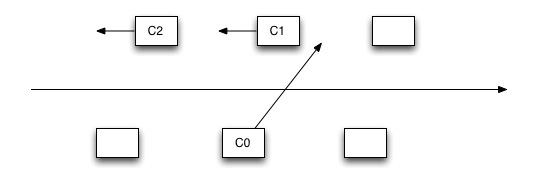
\includegraphics[scale = 0.5]{plot/P1}
\caption{car overtaking illustration of unruled two lane traffic\label{safety1}}

\end{figure}

\begin{figure}
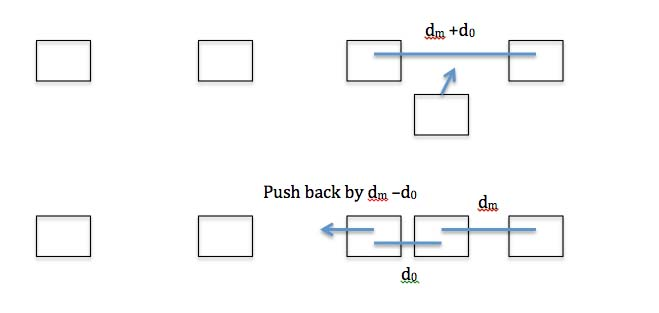
\includegraphics[scale = 0.5]{plot/P2}
\caption{illustration of minimum distance pushed back\label{safety2}}
\end{figure}

From the graphical illustrations(\ref{safety2}), we notice that the car $C_0$ is pushed back by $d_m-d_0$, $C_1$ is pushed back by $d_m-2d_0$ and the $i^{th}$ car is pushed back by $d_m-id_0$. The car $C_i$ will not slow down if $d_m-id_0\le 0$, i.e. $d_m \le id_0$. Therefore, the number of cars slowed down $n \approx d_m/d_0$ when $d_0 << d_m$. 

Thus, we would be able to calculate the total amount of braking distance made by all cars after $C_0$

\begin{align}
&d_t = d_m-d_0 + d_m-2d_0 + \dots + d_m - nd_0 & \\
&d_t = nd_m-\frac{(d_0+nd_0)(n)}{2}&\\
&d_t = \frac{d_m^2}{d_0}-\frac{(d_0+d_m)(d_m)}{2d_0}&\\
&d_t = \frac{d_m^2-d_0d_m}{2d_0}
\end{align}

In particular, if the $d_t \le 0$, i.e. no car needs to slow down, we have $d_m\le d_0$, which means that when the minimum safe distance is less than the extra safe distance, no car will slow down. 

Now, let's take a look at the case if the rule is applied to the two lane traffic situation. In this case, the right lane is the regular lane and the left lane is the passing lane, which suppose to have a higher speed. When a car, $C_0$, is trying to take over the car(s) in front, it needs to shift to the left lane and then shift back to the right lane after overtaking a number of cars. Suppose $C_0$ only overtake one car $C_1$, then when $C_0$ shifts back to the right lane, $C_1$ probably needs a slow down if $d_m>d_0$. However, we notice that because $C_0$ has shifted out of the right lane in the first place, it has left a space of $2(d_s)$ behind $C_1$. Thus, the slow down distance of $C_1$ after $C_0$ has shifted back to the is $d_m-d_0$. Therefore, the distance remain behind $C_1$ after it finished slowing down is

\begin{align}
&2(d_s)-(d_m-d_0)&\\
=\ &2(d_m+d_0)-(d_m-d_0)&\\
=\ &d_m+3d_0&\\
\ge \ &d_m&
\end{align}

Therefore, in this case, $C_1$ is the only affected car. And the slow down distance is $d_m-d_0$

If we increase the number of car that $C_0$ overtakes, we know that the first car overtaken by $C_0$ needs to slow down by $d_m-id_0$, which is less than $d_m+3d_0$. Thus, the maximum number of cars affected is $max(d_m/d_0, i)$. This shows that the number of cars slowed down is no more than the previous case. In addition, the total amount of slow down distance is still

\begin{equation}
d_t = d_m-d_0 + d_m-2d_0 + \dots + d_m - id_0 
\end{equation}
However, since $i\le n$, the total slow down distance is less or equal to the previous case. 


\subsubsection{Safety model on light and heavy traffic comparison}

Now, let's consider the difference between light and heavy traffic. From our assumption, as the traffic density $\rho$ increase, $d_0$ decrease. Therefore, the number of cars slowed down $n\approx d_m/d_0$ is increased. This explains that as the traffic become heavier, the chance for a safety risk is increased. In light traffic, we notice that $d_m \approx d_0$, and then in this case, both situation (ruled and unruled) has no need for slowing down. Thus, the difference in safety issue is insignificant. 


\subsubsection{summary of safety}

In analyzing the safety issue, we used a similar microscope model to determine the relationship between adjacent cars. This is built upon a discreet realization of the kinematic model to simulate and calculate the situation of overtaking in both ruled and unruled traffic. We were able to draw the conclusion that the ruled traffic is better at reducing the safety threat.

\subsubsection{Issue with compliance}

In the previous safety model, we assumed that each one follow the suggested rule by setting the following time $t = 2$ and  the minimum following distance $d \ge vt$. However, in case of low compliance, some people may shorten the following time, thus the following distance. Suppose those cars has a shorter following distance $d_m'$. Because of their lowered following time, the distance between it and the car in front is almost inflexible. Thus, the wave of slowing down would not be tolerant at those cars. The number of cars involved in wave of slowing down would be $n' = d_m/d_0+\alpha$, where $\alpha$ is the number of cars that has shorter following distance $d_m'$. This increase in number of slowing down cars is a potential risk to the safety issue. 